\documentclass[12pt,a4paper,fleqn]{bv_report}


\usepackage{latexsym}
\usepackage{amsmath}
%\usepackage{amssymb}
\usepackage{gensymb}
\usepackage{graphicx}
\graphicspath{{Pictures/}}
\usepackage{subfig}
\usepackage[skip=0pt]{caption}
\usepackage{float}
\usepackage{calc,ifthen,xspace}
%\usepackage{colortbl}
%\usepackage{color}
%\usepackage{xcolor}
\usepackage{fancyhdr}
%\usepackage{bbding}
%\usepackage{wasysym}
\usepackage{hyperref}
%
%\hypersetup{colorlinks, citecolor=black, filecolor=black,  linkcolor=black,  urlcolor=blue}


\usepackage{listings}             % Include the listings-package
\lstdefinestyle{customc}{
  belowcaptionskip=1\baselineskip,
  breaklines=true,
  frame=L,
  xleftmargin=\parindent,
  language=C,
  showstringspaces=false,
  basicstyle=\footnotesize\ttfamily,
  keywordstyle=\bfseries\color{green},
  commentstyle=\itshape\color{purple},
%  commentstyle=\itshape\color{red},
  identifierstyle=\color{blue},
  stringstyle=\color{orange},
}
\lstset{language=C++,style=customc}          % Set your language (you can change the language for each code-block optionally)
\newcommand{\includecode}[2][c]{\lstinputlisting[caption=#2, escapechar=, style=customc]{#2}<!---->}



%For flowcharts
\usepackage[latin1]{inputenc}
\usepackage{color}
\usepackage{tikz}
\usetikzlibrary{shapes,arrows}
\usepackage{tkz-graph}
%%%%%%%%%%%

\usepackage{bm}

\setlength{\parindent}{0.0cm}
\setlength{\parskip}{0.4cm plus3mm minus3mm}

\def\pm{\ ^+_- \ }
\def\mp{\ ^-_+ \ }

\setlength{\oddsidemargin}{0.00cm}
\setlength{\topmargin}{-0.50cm}
\setlength{\textwidth} {16.00cm}
\setlength{\textheight}{23.20cm}



\titrerapport{User guide of foamStar}
\nomaffaire{OpenFOAM}
\noata{ATA 1350A}
\nont{NT 3259}
\reva{0}\datea{March 17th 2017}\writtenbya{Charles Monroy}\objreva{}\checkedbya{}
%\marineconditions


\begin{document}

%\let\start@align@nopar\start@align

\bvpage

\tableofcontents

\clearpage

%\input{macro}

\chapter{Introduction}

This manual aims at explaining how to use foamStar and related pre-processing and post-processing tools.

The theory is covered in a separate document.

The different tools presented for pre-processing and post-processing are accessible in git repository \emph{foamBazar}\footnote{\emph{foamBazar} repository can be found on GitHub : https://github.com/cmonroy}.

%A separate document will be written concerning user guide and best practice.


%verification, validation

\chapter{Installation}


\section{Mandatory packages for foamStar}

It is necessary to install Lapack on the platform.
\begin{lstlisting}[language=bash]
  $ sudo apt-get install liblapack-dev liblapack-doc-man liblapack-doc liblapack-pic liblapack3 liblapack-test liblapack3gf liblapacke liblapacke-dev
\end{lstlisting}


\chapter{Automatic generation of a mesh for sea-keeping}

The CFD mesh for sea-keeping can be generated by several methods. The most common uses standard OpenFoam tools such as \emph{snappyHexMesh} but STAR-CCM+ mesh generator can be used for tricky geometries.

\section{Body geometry}

Geometry of the body (ship) must be handled with care. Since most finite element meshes doesn't provide fine enough description of the hull, it is advised to start directly from the hull geometry (IGES file or other).

CFD meshing tools require a geometry in stereolithography format (.stl), this file can be created using standard meshing software such as FEMAP or Gmsh. Please note that STL geometry must particularly be refined in curved areas such as bow and stern parts in order to precisely represent actual hull geometry. IGES and STL samples are presented in Fig. \ref{geom}.

\begin{figure}[htbp]
\begin{center}
\subfloat[Geometries in IGES (top) and STL (bottom) formats]{
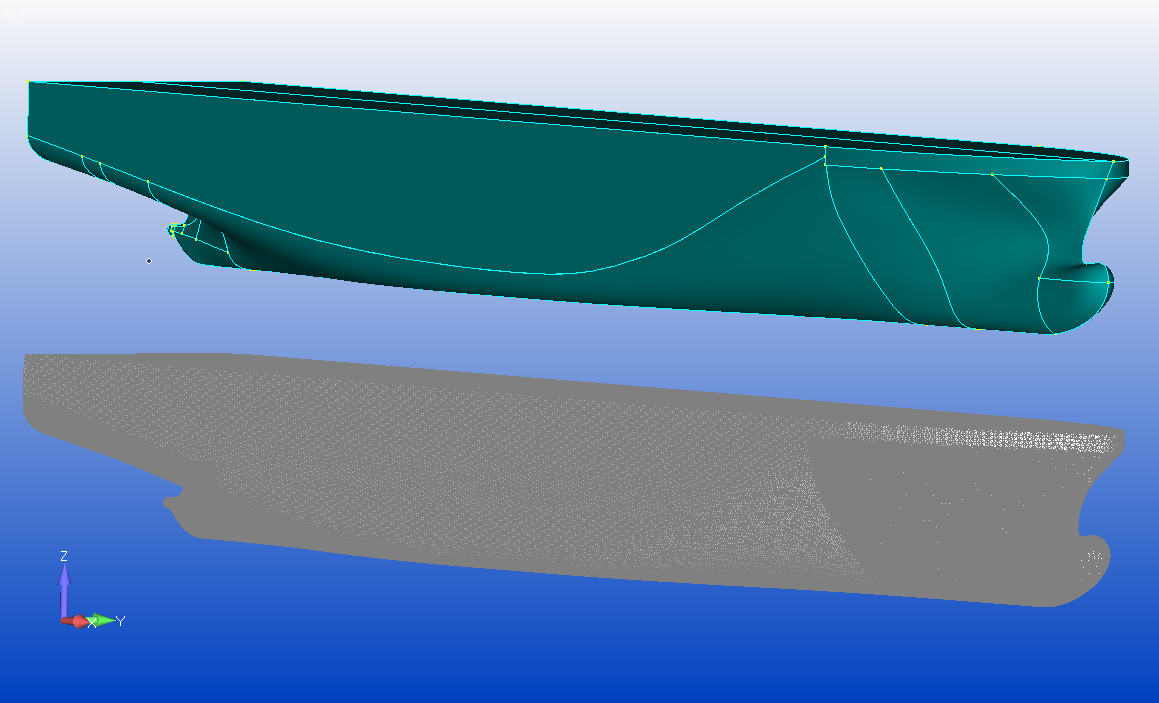
\includegraphics[width=8.5cm]{igs_stl.png}
\label{geom1}
}
\subfloat[STL refinement in bow area]{
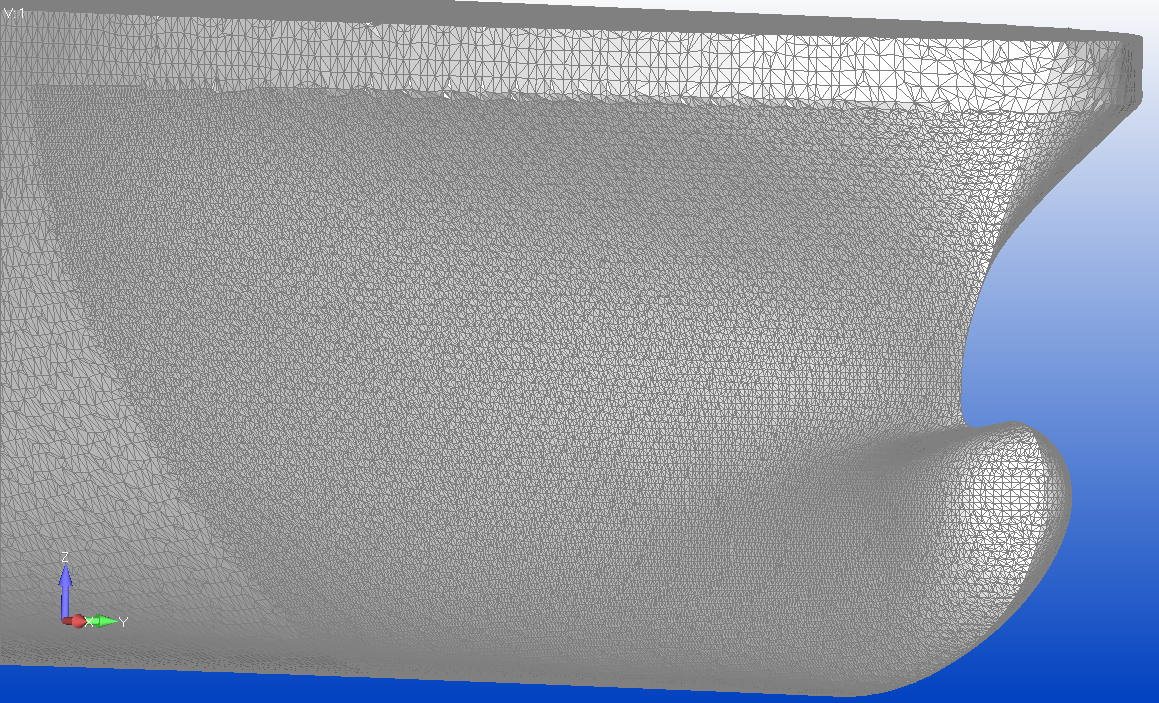
\includegraphics[width=8.5cm]{fine_stl.png}
\label{geom2}
}
\end{center}
\caption{Body geometry}
\label{geom} 
\end{figure}

\section{CFD mesh generation (fsMesher)}

A python script has been developed for convenient CFD mesh generation with OpenFoam tools,  it can be found in \emph{foamBazar} repository. This script works with an input file described hereafter.

\subsection{fsMesher input file}

Input file for fsMesher python scipt contains all information needed for automatic CFD mesh generation, the corresponding extension is .cfg. A template can automatically be created using the following command:
\begin{lstlisting}[language=bash]
$ fsMesher.py -p
\end{lstlisting}

Input file options are described hereafter:
\paragraph{STL geometry file}
Multiple non-overlapping STL geometry files can be used to define the body. A specific patch will be created for each STL file. At least one file must be defined:
\begin{lstlisting}[language=bash]
# STL geometry files
stlFile0 = ./body.stl
stlFile1 = ./deck.stl
stlFile2 = ./stern.stl
\end{lstlisting}

\paragraph{Draft}
Draft must be defined from keel in the STL file coordinates system. If different from zero, the geometry is moved relatively to free surface.
\begin{lstlisting}[language=bash]
# Draft (measured from keel)
draft = 15.0
\end{lstlisting}

\paragraph{Refinement in areas with strong curvature}
Areas with strong curvature such as bow and stern parts can be specified in order to be refined automatically. User must provide these areas in STL format.
\begin{lstlisting}[language=bash]
# Extra refinement in bow/stern areas with strong curvatures
refineSurf = kcs-curves.stl
\end{lstlisting}

\paragraph{Draft}
Draft must be defined from keel in the STL file coordinates system. It can be set to "None" if the geometry is already in correct position, otherwise the geometry will be moved relatively to free surface.
\begin{lstlisting}[language=bash]
# Draft (measured from keel)
draft = 15.0
\end{lstlisting}

\paragraph{Heading}
Heading is defined in degrees by the following parameter, 180\degree  corresponds to head sea.
\begin{lstlisting}[language=bash]
# Heading (in degrees)
heading = 180
\end{lstlisting}

\paragraph{Side to mesh}
In case of head sea, only one half of the domain has to be meshed, this parameter is use to select which side must be considered ("port" or "starboard"). In case of non-symmetrical mesh, the option "both" should be used.
\begin{lstlisting}[language=bash]
# Side : port, starboard or both ?
side = port
\end{lstlisting}

\paragraph{Domain size}
The size of the whole CFD domain is defined in relation with ship overall length (LOA). Six coefficients ($c_1$, ..., $c_6$) must be defined to set domain boundaries such as $X_{min}= c_1 \cdot \text{LOA}$, $X_{max}= c_2 \cdot \text{LOA}$, $Y_{min}= c_3 \cdot \text{LOA}$, $Y_{max}= c_4 \cdot \text{LOA}$, $Z_{min}= c_5 \cdot \text{LOA}$ and $Z_{max}= c_6 \cdot \text{LOA}$. Default values (-3.0, 2.5, -2.0, 2.0, -0.82124, 0.5555) can be used by setting the keyword to "auto".
\begin{lstlisting}[language=bash]
# Domain size relatively to LOA [X(min,max) Y(min,max) Z(min,max)]
domain = -3.0, 2.5, -2.0, 2.0, -0.82124, 0.5555
\end{lstlisting}

\paragraph{Characteristic length}
Overall length (LOA) is usually directly computed from the geometry ("auto") but it can also be user-defined with this parameter.
\begin{lstlisting}[language=bash]
# Characteristic length
LOA = 300.
\end{lstlisting}

\paragraph{Free surface zone}
The vertical extent of the free surface refined zone is defined in relation with ship overall length (LOA). Two coefficients ($c_1$, $c_2$) must be defined to set domain boundaries such as $Z_{min}= -c_1 \cdot \text{LOA}$ and $Z_{max}= c_2 \cdot \text{LOA}$. Default values (0.02, 0.01) can be used by setting the keyword to "auto".
\begin{lstlisting}[language=bash]
# Free surface zone relatively to LOA [Z(min,max)]
fsZone = 0.02, 0.01
\end{lstlisting}

\paragraph{Cell height within the free surface zone}
Cell height in free surface zone can be defined with this parameter. Default value (0.33*fsZmax) can be used by setting the keyword to "auto".
\begin{lstlisting}[language=bash]
# Cell height within the free surface zone
fsCellHeight = 1.5
\end{lstlisting}

\paragraph{Cell ratio length/height within the free surface zone}
Cell ratio  length/height in free surface zone can be defined with this parameter. Default value (4) can be used by setting the keyword to "auto".
\begin{lstlisting}[language=bash]
# Cell ratio length/height within the free surface zone
fsCellRatio = 4
\end{lstlisting}

\paragraph{Type of refinement box(es) in the domain}
The type of refinement boxes can be defined with the following parameter. Available options are "wave", "kelvin" or "both".
\begin{lstlisting}[language=bash]
# Type of refinement box(es) in the domain
refBoxType = wave
\end{lstlisting}

\paragraph{Data for refinement boxes}
Refinement boxes can be defined in an automatic and manual way. The automatic way requires definition of two parameters: "refBoxData" and "refBoxRatio". The fist corresponds to the number of refinement boxes and the second to the ratio between the smallest and the largest boxes. Default values (3 for both parameters) can be used for automatic refinement by setting the keywords to "auto". Refinement boxes can also be defined manually with parameter "refBoxData" followed by the number of boxes and the corresponding coordinates in X-Y plane $X_{min}$, $X_{max}$, $Y_{min}$, $Y_{max}$ for each box.
\begin{lstlisting}[language=bash]
# Automatic definition of refinement box(es) in the domain
refBoxData = 3
refBoxRatio = 3

# Manual definition of refinement box(es) in the domain
# NbBox, Xmin1, Xmax1, Ymin1, Ymax1, Xmin2, Xmax2, Ymin2, Ymax2, ... 
refBoxData = 2, -500, 600, -50, 350, -250, 600, -50, 350 
\end{lstlisting}

\paragraph{Cell buffer between refinement level}
In order to avoid brutal refinement between each zone, a minimal number of cells can be defined between two zones. Default value (4) can be used by setting the keyword to "auto".
\begin{lstlisting}[language=bash]
# Cell buffer between refinement level
cellBuffer = 4
\end{lstlisting}

\paragraph{Additional refinement at the bow and stern regions}
Additional refinement in bow and stern areas can be defined with this parameter. Such refinements are particularly used to improve slamming accuracy in these zones. Refinement boxes size are defined by a coefficient relatively to LOA. Bow and sterm refinements can be disabled by setting these parameters to zero. Default values (0.2) can be used by setting the keyword to "auto".
\begin{lstlisting}[language=bash]
# Additional refinement at the bow region
refineBow = 0.2

# Additional refinement at the stern region
refineStern = 0.2
\end{lstlisting}

\paragraph{Additional vertical refinement in the free surface zone near the ship}
Additional vertical refinement around the free surface in the ship area can be defined with this parameter. The value can be "True" or "False".
\begin{lstlisting}[language=bash]
# Additional vert. refinement in the free surface zone near the ship
refineFS = False
\end{lstlisting}

\paragraph{Dimensions of boundary layers}
Boundary layers can be defined around the body using this parameter. Default values can be used by setting the keyword to "auto". The following values must be defined:
\begin{itemize}
\item number of layers (default=3)
\item layer growth (default=1.3)
\item thickness of final boundary layer (default=0.7)
\item minimal thickness ratio (default=0.7)
\end{itemize}
\begin{lstlisting}[language=bash]
# Dimension for boundary layers (relative to cell size)
# nLayers, layerGrowth, finalLayerThickness, minThicknessRatio
layers = 3, 1.3, 0.7, 0.7
\end{lstlisting}

\paragraph{Disable location for selected patch}
Boundary layers are created on all patches by default but can be removed from some of them is not needed (e.g. it is usually not needed on deck). The name(s) of patch(es) to be removed from boundary layer must be given (separated by commas).
\begin{lstlisting}[language=bash]
# Deactivate boundary layer on patch(es)
disableLayers = deck
\end{lstlisting}

\paragraph{Additional setting}
Follonwig additional settings can be added to input file:

\begin{lstlisting}[language=bash]
# these are optional settings for fsMesher.py
[fsMesher-control]

# these switches can be called from command line
# settings called from command line overrule settings in this config-file
# note: NPROCS has no effect when "system/decomposeParDict" exists
DEBUG = True
NPROCS = 4
EXEC_BLOCKMESH = True
EXEC_REFINEBOX = True
EXEC_REFINEPROXIMITY = True
EXEC_SNAP = True
EXEC_ADDLAYERS = True

# main stl-filename in "./constant/triSurface/"
DEFAULT_SHIP_STL = ship.stl

# Self-explained settings ... 
# log-file for foam tools is defined in CMD_keepLog.
# output from python script is flushed to stdOut
CMD_keepLog = ' >> ./log.fsMesher 2>&1 '
CMD_showLog = 'echo "\nlog-file: ./log.fsMesher"; tail -45 ./log.fsMesher; echo "Please see log-file: ./log.fsMesher"'
CMD_blockMesh = 'blockMesh'
CMD_autoPatch = 'autoPatch -overwrite 80'
CMD_setSet = 'setSet -latestTime'
CMD_refineMesh = 'refineMesh'
CMD_snappyHexMesh = 'snappyHexMesh'
CMD_decomposePar = 'decomposePar -force -latestTime'
\end{lstlisting}

\subsection{Launch fsMesher}

Before generating the CFD mesh , it can be useful to check the commands that will be executed by fsMesher script. This can be done by using "-n" option. The results can also be stored in a log file unsing this command :
\begin{lstlisting}[language=bash]
$ fsMesher.py -f fsMesher.cfg -n > log.dryrun
\end{lstlisting}

The script can then be executed with :
\begin{lstlisting}[language=bash]
$ fsMesher.py -f fsMesher.cfg
\end{lstlisting}

Once finished, if parallel computation has been used, one need to reconstruct the data using the following command:
\begin{lstlisting}[language=bash]
$ reconstructParMesh
\end{lstlisting}

The resulting meshes can be found in time folders, the higher value corresponds the final mesh and others are intermediate steps. Meshes can directly be viewed with Paraview (Windows users should insert a void "*.foam" file to use with Paraview).

\begin{figure}[htbp]
\begin{center}
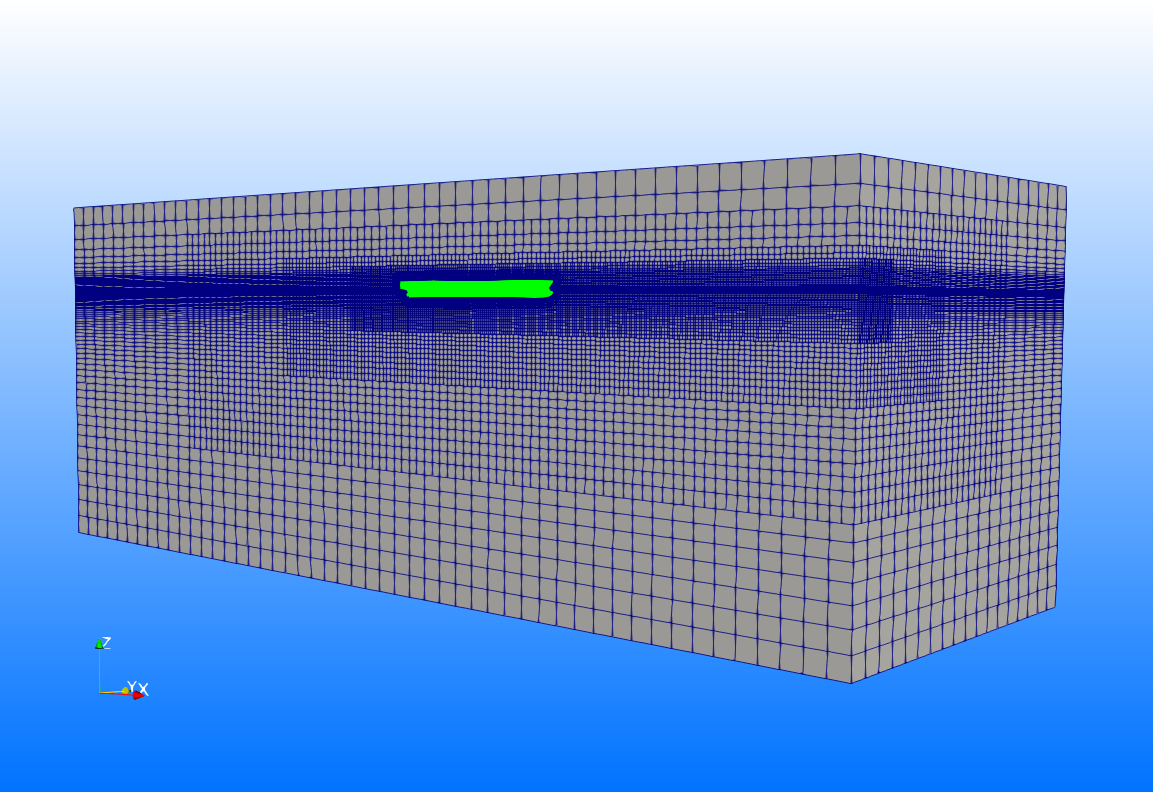
\includegraphics[width=12cm]{CFD_mesh.png}
\end{center}
\caption{CDF mesh with ship}
\label{cfd_mesh} 
\end{figure}


\subsection{Recommendations for mesh generation}

Here are summarized some common advise for mesh quality:
\begin{itemize}
\item Number of cell in X-direction should be at least 100 per wave length
\item Symmetry plane has to be defined on patch Y0 for head seas. It is advised to add another symmetry plane on patch Y1 for high forward speed cases
\item All body patches created by fsMesher (hull, deck, ...) should be merged into one single patch manually or using \emph{createPatch}
\end{itemize}


\cite{Shabana1989}

\chapter{Pre-computing structural information}
\label{homer}

All structural information needed for mechanical equation solving and flexible modes can be pre-computed from an Homer 2 model.

\section{Running Homer}
Once the model has been set up, HmFEM has to be run with the following body options. Please refer to Homer user guide for more information about Homer keywords.

\begin{lstlisting}[language=fortran]
# Strcutural mesh information
STRUCTURALMESH = body.dat
STRUCTURALCOORDINATES = 0. 0. -11.75 0. 0. 0.
STRUCTURALLENGTHUNIT = m
STRUCTURALMASSUNIT = kg

# Number of flexible modes if required
STRUCTURALNFLEXIBLEMODES = 3

# Enable specific outputs for OpenFoam
PREPAREOPENFOAM = 1

# Sections definition
SECTIONS
CUT   -6.00 0. 12.015 1. 0. 0.
CUT   82.83 0. 12.015 1. 0. 0.
CUT  150.78 0. 12.015 1. 0. 0.
CUT  223.23 0. 12.015 1. 0. 0.
CUT  295.00 0. 12.015 1. 0. 0.
ENDSECTIONS
\end{lstlisting}

HmFEM will then run normally and create the following files that are useful for foamStar:
\begin{itemize}
\item mesh : Finite\_Elements\_Analysis{\textbackslash}HmFEM{\textbackslash}\textbf{body\_Bulk.dat}
\item mass matrix : Finite\_Elements\_Analysis{\textbackslash}HmFEM{\textbackslash}\textbf{body\_dmig.pch}
\item mode shapes : Finite\_Elements\_Analysis{\textbackslash}HmFEM{\textbackslash}\textbf{body\_md.pch}
\item don file : User\_Outputs{\textbackslash}HmFEM{\textbackslash}\textbf{body.don}
\end{itemize}

\section{Initialize structural information for foamStar}

Structural data pre-processing for foamStar is performed using the module \emph{initFlx} together with a standard OpenFoam input file \emph{initFlxDict} described hereafter:

\begin{lstlisting}[language=C]
FEM_STRUCTURALMESH_VTU
{
    datFile "body_Bulk.dat";
    mdFile "body_md.pch"; selected (7 8 9);
    dmigMfile "body_dmig.pch";
    dmigKfile "body_dmig.pch";
    pchCoordinate (0 0 -11.75 0 0 0);
    pchScaleMode  0.25909281809220411E+05;
    pchLengthUnit 1;
    pchMassUnit   1;

    patches (ship); ySym (true);
}
\end{lstlisting}

\begin{itemize}
\item \textbf{datFile} : finite element mesh provided by Homer (*\_Bulk.dat)
\item \textbf{mdFile} : modes shapes punch file given by Homer (*\_md.pch)
\item \textbf{selected} : select flexible modes to use for simulation (starting from mode 7)
\item \textbf{dmigMfile} : mass matrix punch file provided by Homer (*\_dmig.pch)
\item \textbf{dmigKfile} : stiffness matrix punch file provided by Homer (*\_dmig.pch)
\item \textbf{pchCoordinate} : structural coordinates used in Homer
\item \textbf{pchScaleMode} : value of scaling factor of first mode in Homer
\item \textbf{pchLengthUnit} : length scaling factor to meters (m=1, mm=0.001)
\item \textbf{pchMassUnit} : mass scaling factor to kilograms (kg=1, t=1000)
\item \textbf{pchMassUnit} : mass scaling factor to kilograms (kg=1, t=1000)
\item \textbf{patches} : define patch representing the hull
\item \textbf{patches} : define if Y-symmetry is used or not
\end{itemize}

foamStar module can then be launched with the following command:
\begin{lstlisting}[language=bash]
$ initFlx
\end{lstlisting}






\chapter{FoamStar data setup}

\section{Mesh}

The mesh should be prepared in a separate folder from the calculation folder (cf. part \ref{mesh}). Once created the mesh can be transferred to the calculation folder by hand or using fsTemplate python script described hereafter.

\section{Using fsTemplate.py}

All inputs for foamStar correspond to text files that can be written manually. Howerver, due to the huge number of files and options, it is easier and safer to use a template. The fsTemplate.py is a specific script written for automatic foamStar case generation, all parameters need to be set in an input file described hereafter.

\subsection{fsTemplate input file}

Input file for fsTemplate python script contains all information needed for automatic foamStar case generation, the corresponding extension is .cfg. A template can automatically be created using the following command:
\begin{lstlisting}[language=bash]
$ fsTemplate.py -p
\end{lstlisting}

Input file options are described hereafter:

\paragraph{Case name}
The case name, also used as directory name and job name should be given as follow.
\begin{lstlisting}[language=bash]
#Set name of case folder to be created
caseDir = myCase
\end{lstlisting}

\paragraph{Mesh}
The mesh location should be given with the following keywords. The mesh directory (relative path) should be provided together with the time folder to be used. The final mesh can be selected automatically by setting "meshTime = latestTime".
\begin{lstlisting}[language=bash]
#Set location of mesh folder, stl file name and time folder from which it should be retrieved ('0.08', '0.09' or 'latestTime')
meshDir = mesh
meshTime = latestTime
\end{lstlisting}

\paragraph{STL}
The name of STL file containing the hull and used to generate the mesh should be given as follow. This file should be located in "meshDir/constant/triSurface" folder.
\begin{lstlisting}[language=bash]
#Set name of stl file
stlFile = ship.stl
\end{lstlisting}

\paragraph{Hull patch name}
The name to be given to the hull patch should be provided with the following keyword.
\begin{lstlisting}[language=bash]
#Set patch name given for hull in boundary file
hullPatch = ship
\end{lstlisting}

\paragraph{Solver parameters}
Basic solver parameters such as the solver selections, the number of processors to be used in parallel and the scheme (Euler or Chrank Nicolson) can be defined as follow.
\begin{lstlisting}[language=bash]
#Set OpenFOAM solver parameters 
solver = foamStar
nProcs = 24
scheme = Euler
\end{lstlisting}

\paragraph{Case control}
Parameters controlling the case can be defined as follow. It includes:
\begin{itemize}
\item Start time of simulation
\item End time of simulation
\item Time step of simulation
\item Write interval of full output (warning: these outputs takes a lot of disk space)
\item Number of full outputs to be kept (keep last N output time steps)
\item Outputs controls (global motions, local motions, internal loads and wave probes)
\item Local motion points definition (if local motions are needed)
\item Wave probes location definition (if wave probes are needed)
\item Tolerance to be used for CFD solver iterations
\end{itemize}

\begin{lstlisting}[language=bash]
#Set case control parameters
startTime = latestTime
endTime = 4000
timeStep = 0.05
writeInterval = 40
purgeWrite = 5
outputMotions = True
localMotionPts = X1 Y1 Z1; X2 Y2 Z2; X3 Y3 Z3
outputVBM = True
outputWave = False
waveProbes = xMin Xmax nX y zMin zMax nZ; xMin Xmax nX y zMin zMax nZ
fsiTol = 1e-6
\end{lstlisting}

\paragraph{Wave properties}
Parameters controlling the wave can be defined as follow. It includes:
\begin{itemize}
\item Wave type (noWaves, streamFunction, ...)
\item Water depth
\item Draft
\item Forward speed
\item Wave height (regular wave only)
\item Wave period (regular wave only)
\item Sea level
\item Wave start time 
\item Wave ramp time
\item Additional hydrodynamic damping (to be used for faster still water cases convergence)
\end{itemize}

\begin{lstlisting}[language=bash]
#Set wave properties
wave = noWaves
depth = 500
draft = 0
velocity = 0.0
waveH = 1.0
waveT = 10.0
waveSeaLvl = 0
waveStartTime = 0
waveRampTime = 10
addDamping = False
\end{lstlisting}

\paragraph{Relaxation zones}
Relaxation zones can be defined to blend the wave at input, output or on the sides of the domain. Theses zones are used to avoid reflections on the boundaries and ensure a clean wave field around the ship. These zones are defined by two boundaries, the first is one of the domain boundary and the other has to be user-defined. It corresponds to X, Y or Z coordinates depending on zone type.
\begin{lstlisting}[language=bash]
#Set Relaxation zones (set 0 if no zone)
inletRelaxZone  = 400
outletRelaxZone = -250
sideRelaxZone   = 250
\end{lstlisting}

\begin{figure}[htbp]
\begin{center}
    \def\setA{(0,0) circle (1)}
    \def\setB{(0,0) circle (1)}
    
    \begin{tikzpicture}
        % Top view
        \draw (-8,2) rectangle (8,-2);
        \draw[fill=black!25] (-2,-2) -- (-2,-1.5) .. controls (1.3,-1.5) and (1.5,-1.5) .. (2,-2) -- (-2,-2);
        
        \draw[red,dashed] (4,2) -- (4,-2);
        \fill [pattern color=red, pattern=north east lines] (4,2) -- (8,2) -- (8,-2) -- (4,-2);
        \node at(6,0) [draw,fill=white,opacity=.8,text opacity=1] {Inlet zone};
        \draw[red,dashed] (-3,2) -- (-3,-2);
        \fill [pattern color=red, pattern=north east lines] (-3,2) -- (-8,2) -- (-8,-2) -- (-3,-2);
        \node at(-5.5,0) [draw,fill=white,opacity=.8,text opacity=1] {Outlet zone};
        \draw[purple,dashed] (-8,0.5) -- (8,0.5);
        \fill [pattern color=purple, pattern=north west lines] (-8,2) -- (-8,0.5) -- (8,0.5) -- (8,2);
        \node at(0,1.25) [draw,fill=white,opacity=.8,text opacity=1] {Side zone};
        
    \end{tikzpicture}
\end{center}
\caption{Relaxation zones}
\label{boundaries} 
\end{figure}

\paragraph{Scheme blending}
When using Crank Nicolson scheme, instabilities appears around the floating body. This can bypassed by using Euler scheme around the body. The size of the zone where Euler scheme will be used can be set with following parameter providing the distance between the body and the zone boundary.
\begin{lstlisting}[language=bash]
#Set Euler zones (set 0 if no zone)
EulerCellsDist  = 8
\end{lstlisting}

\begin{figure}[htbp]
\begin{center}
    \def\setA{(0,0) circle (1)}
    \def\setB{(0,0) circle (1)}
    
    \begin{tikzpicture}
        % Top view
        \draw (-8,2) rectangle (8,-2);
        \draw[purple] (-2.4,-2) -- (-2.4,-1.2) .. controls (1.625,-1.2) and (1.875,-1.2) .. (2.4,-2);
        \fill [pattern color=black!50, pattern=dots] (-8,2) rectangle (8,-2);
        \fill [pattern color=purple, pattern=north east lines] (-2.4,-2) -- (-2.4,-1.2) .. controls (1.625,-1.2) and (1.875,-1.2) .. (2.4,-2) -- (-2.4,-2);
        \draw[fill=black!25] (-2,-2) -- (-2,-1.5) .. controls (1.3,-1.5) and (1.5,-1.5) .. (2,-2) -- (-2,-2);
        
        \node at(0,1) [fill=white] {Crank Nicolson scheme};
        \node at(3,-1) [right,purple,fill=white,draw] {Euler scheme};
        \draw[purple] (3,-1) -- (2,-1.55);

    \end{tikzpicture}
\end{center}
\caption{Scheme blending}
\label{boundaries}
\end{figure}

\paragraph{Structural data}
Structural data including mass distribution and flexible properties have to be provided using the following keywords. The corresponding files are described in part \ref{homer}.  It includes:
\begin{itemize}
\item A DAT file containing the mesh
\item A DON file containing information about the sections
\item A DMIG file with mass matrix
\item A MD file with informations about flexible modes
\item Homer HmFEM output file with standard information
\item Flexible modes to be used
\item Structural damping to be added on each flexible mode
\end{itemize}

\begin{lstlisting}[language=bash]
#Set structural data obtained with Homer
#all path should be written relatively to this input file location
datFile =  ../homer/ship.dat
donFile = ../homer/ship.don
dmigfile = ../homer/ship_dmig.pch
mdFile = ../homer/ship_md.pch
hmrUserOutput = ../homer/HmFEM.out
modesToUse = 7 8 9
shipDamping = 0.01 0.01 0.01
\end{lstlisting}


\subsection{Launch options}

To run the fsTemplate.py python script, the following command should be used with the input file described previously:
\begin{lstlisting}[language=bash]
fsTemplate.py -f inputFile.cfg
\end{lstlisting}

This script can generate all inputs files for foamStar but can also initialize the case by running corresponding foamStar routines. The following options are available:
\begin{itemize}
\item \textbf{-i}: initialize the foamStar case (generate zones, initialize wave field and initialize flexible modes)
\item \textbf{-d}: run the decomposition of the case for parallel run
\item \textbf{-tar}: creates an archive file with the case ready to be launched
\end{itemize}


\chapter{Log analyzer}

\section{Useful shell commands}

\begin{lstlisting}[language=bash]
  $ grep -E "^Time =|Cour" log.run | less
\end{lstlisting}

\begin{lstlisting}[language=bash]
  $ grep -E "^Time =|p_rgh|PIMPLE" log.run | less
\end{lstlisting}

\section{fsAwk}

You first need to make symbolic links in /bin to python scripts. To do this:

\begin{lstlisting}[]
  $ cd ~/bin
  $ ln -s ~/dvt/foamBazar/pythonScripts/fsLog.awk .
  $ ln -s ~/dvt/foamBazar/pythonScripts/fsPlot.py . 
\end{lstlisting}

When typing \textit{fsPlot.py} and relative input,it will automatically parse the log file through the script "fsAwk" (if it is not done already). All the possible commands of \textit{fsPlot.py} are listed through the help command.
\begin{lstlisting}[language=bash]
  $ fsPlot.py --help
\end{lstlisting}

Below are some examples, based on a log file called "\textit{log.run}".
\begin{itemize}
\item Plot the time history of all the different Courant numbers (max and mean of flow and interface Courant numbers):
\begin{lstlisting}[language=bash]
  $ fsPlot.py -p co log.run
\end{lstlisting}

\item Plot the time history of maximum of flow Courant number:
\begin{lstlisting}[language=bash]
  $ fsPlot.py -p co -w max log.run
\end{lstlisting}

\item Plot the time history of maximum of interface Courant number:
\begin{lstlisting}[language=bash]
  $ fsPlot.py -p co -w max,interface log.run
\end{lstlisting}

\item Plot the time history of the initial residual of Ux:
\begin{lstlisting}[language=bash]
  $ fsPlot.py -p res -w init,Ux log.run
\end{lstlisting}

\item Plot the time history of the force in the z-direction at the final iteration:
\begin{lstlisting}[language=bash]
  $ fsPlot.py -p f -w z log.run
\end{lstlisting}

\item Plot the time history of the force in the z-direction at all iterations:
\begin{lstlisting}[language=bash]
  $ fsPlot.py -p f -w z -i
\end{lstlisting}

\item Plot the time history of the force in the z-direction at all iterations with markers:
\begin{lstlisting}[language=bash]
  $ fsPlot.py -p f -w z -i -l s:-,m:x
\end{lstlisting}

\end{itemize}


\chapter{Using Liger cluster}

\section{Setting up environment}

You can find some useful settings in /data/I1608251/forNewComersToLiger. You can copy them to your home directory:

\begin{lstlisting}[language=bash]
  $ cd
  $ mkdir bin 
  $ cp /data/I1608251/forNewComersToLiger/settings bin/
\end{lstlisting}

And edit your .bashrc in your home folder by adding the line at the end of the file:
\begin{lstlisting}[language=bash]
  $ . /bin/settings
\end{lstlisting}

In this way, you will be able to source different OpenFOAM versions by the commands:
\begin{lstlisting}[language=bash]
  $ of2.4.x
\end{lstlisting}
or
\begin{lstlisting}[language=bash]
  $ of3.0.x
\end{lstlisting}

In order to benefit from Python environment, you need to add the following line in your path (it is suggested to add this line in your bashrc file):
\begin{lstlisting}[language=bash]
export PATH="/data/I1608251/anaconda2/bin:$PATH"
\end{lstlisting}

\section{Running a batch}

A batch "run.sh" for foamStar looks like this:
\begin{lstlisting}[language=bash]
#!/bin/bash -l
#SBATCH -J fs-KCS-pureEuler

# 5 hour wall-clock 
#SBATCH --account I1608251
#SBATCH -t 3-00:00:00
#SBATCH -n 72
#SBATCH -o log.run-%j

module load gcc/4.9.3 openmpi/1.8.4-gcc lapack/3.6.1/gcc/4.9.3
export FOAM_INST_DIR=/data/I1608251/OpenFOAM;
source /data/I1608251/OpenFOAM/OpenFOAM-2.4.x/etc/bashrc;
export LC_ALL=C

mpirun foamStar -parallel
\end{lstlisting}
You have to make sure that you change the name of the job (here "fs-KCS-pureEuler") and the number of processors (here 72) accordingly to your simulation.

To run the batch, the command is:
\begin{lstlisting}[language=bash]
  $ sbatch run.sh
\end{lstlisting}


To show the queue:
\begin{lstlisting}[language=bash]
  $ squeue
\end{lstlisting}

And to show only your queue (with your own username):
\begin{lstlisting}[language=bash]
  $ squeue | grep userName
\end{lstlisting}


To cancel the job, the command is:
\begin{lstlisting}[language=bash]
  $ scancel jobID
\end{lstlisting}


\section{Keeping alive}

You will get disconnected if you are inactive for more than 5 minutes. In order no to lose your connection (your location and your history - note: you can keep your history with screen), you can use a small trick by defining a keepAlive function in your .bashrc.


\begin{lstlisting}[language=bash]
alias keepAlive='while [ true ]; do clc; date; i=$[(RANDOM % 100)+10]; sleep $i; done'
\end{lstlisting}

You will have to launch "keepAlive" every time you are not working on your session.

\section{Administration}

To know the groups you belong to:
\begin{lstlisting}[language=bash]
groups
\end{lstlisting}

In order to know the CPU hours by everyone of the group:
\begin{lstlisting}[language=bash]
sreport cluster AccountUtilizationByUser start=2016-01-01 accounts=I1608251 -t hours
\end{lstlisting}


%\input{equations}


%\input{logicalSchemes}

%\input{flowSolver}

%\input{sixDofMechanicalSolver}

%\input{modalMechanicalSolver}


%\chapter{Mesh computation}

%\input{FSIinteractions}


%\input{schemes}


%\input{postProcessing}

%\bibliographystyle{plain}

%\bibliography{foamStar_biblio}


\end{document}


